%%%%%%%%%%%%%%%%%%%%%%%%%%%%%%%%%%%%%%%%%%%%%%%%%%%%%%%%%%%%%%%%%%%%%%
%% Copyright (c) 2016 Carsten Wulff Software, Norway
%% %%%%%%%%%%%%%%%%%%%%%%%%%%%%%%%%%%%%%%%%%%%%%%%%%%%%%%%%%%%%%%%%%%%
%% Created       : wulff at 2016-11-5
%% %%%%%%%%%%%%%%%%%%%%%%%%%%%%%%%%%%%%%%%%%%%%%%%%%%%%%%%%%%%%%%%%%%%
%% This program is free software: you can redistribute it and/or modify
%% it under the terms of the GNU General Public License as published by
%% the Free Software Foundation, either version 3 of the License, or
%% (at your option) any later version.
%%
%% This program is distributed in the hope that it will be useful,
%% but WITHOUT ANY WARRANTY; without even the implied warranty of
%% MERCHANTABILITY or FITNESS FOR A PARTICULAR PURPOSE.  See the
%% GNU General Public License for more details.
%%
%% You should have received a copy of the GNU General Public License
%% along with this program.  If not, see <http://www.gnu.org/licenses/>.
%%%%%%%%%%%%%%%%%%%%%%%%%%%%%%%%%%%%%%%%%%%%%%%%%%%%%%%%%%%%%%%%%%%%%%
%\documentclass[final,11pt]{IEEEtran}
\documentclass[crop,border=0pt]{standalone}
\usepackage{times}


%\usepackage{placeins}
\usepackage{upgreek}
\usepackage{amssymb,amsmath}
\usepackage{cite}
\usepackage{verbatim}
\usepackage{listings}
\usepackage{xcolor}
\usepackage{flafter}
\usepackage{booktabs}
\usepackage{url}
\usepackage{ textcomp }

\hyphenation{op-tical net-works semi-conduc-tor}


% -JSON styel

%\definecolor{darkGreen}{rgb}{0,0.2097,0}
%\newcommand{\myfigwidth}{\linewidth}
%\newcommand{\myfigwidtha}{\linewidth}
%\newcommand{\myfigwidthl}{\textwidth}
%\newcommand{\myfigwidthc}{0.6\linewidth}


\newcommand{\myfigwidtha}{3.3in}
\newcommand{\myfigwidthl}{7in}
\newcommand{\myfigwidthc}{2in}
%\newcommand{\myfigwidthe}{3.2in}
%\newcommand{\myfigwidthb}{5in}

\newcommand{\myfigname}{fig_}
\newcommand{\reg}[2]{{\figurename} \ref{#1}(#2)}
\newcommand{\req}[1]{{\figurename} \ref{#1}}
%\newcommand{\myeqname}{eq:}
%\newcommand{\req}[1]{(\ref{\myeqname#1})}

\definecolor{armygreen}{rgb}{0, 0.5, 0}
\newcommand{\missing}[1]{{ #1}}
\newcommand{\edit}[1]{{ #1}}
\newcommand{\secedit}[1]{{ #1}}
\newcommand{\deleted}[1]{{ #1}}
\newcommand{\moved}[1]{{ #1}}

%\newcommand{\missing}[1]{{\color{red} #1}}
%\newcommand{\edit}[1]{{\color{red} #1}}
%\newcommand{\secedit}[1]{{\color{armygreen} #1}}
%\newcommand{\deleted}[1]{{\color{violet} #1}}
%\newcommand{\moved}[1]{{\color{blue} #1}}

\newcommand{\SD}{Sigma-Delta }
\newcommand{\eqn}[1]{
  \begin{math}
    #1
  \end{math}}

\newcommand\JSONnumbervaluestyle{\color{blue}}
\newcommand\JSONstringvaluestyle{\color{red}}



\newif\ifcolonfoundonthisline

\makeatletter

\lstdefinestyle{json}
{
  showstringspaces    = false,
  keywords            = {false,true},
  alsoletter          = 0123456789.,
  morestring          = [s]{"}{"},
  stringstyle         = \ifcolonfoundonthisline\JSONstringvaluestyle\fi,
  MoreSelectCharTable =%
  \lst@DefSaveDef{`:}\colon@json{\processColon@json},
  basicstyle          = \fontsize{7}{7}\ttfamily,
  keywordstyle        = \fontsize{7}{7}\ttfamily\bfseries,
}

% flip the switch if a colon is found in Pmode
\newcommand\processColon@json{%
  \colon@json%
  \ifnum\lst@mode=\lst@Pmode%
  \global\colonfoundonthislinetrue%
  \fi
}

\lst@AddToHook{Output}{%
  \ifcolonfoundonthisline%
  \ifnum\lst@mode=\lst@Pmode%
  \def\lst@thestyle{\JSONnumbervaluestyle}%
  \fi
  \fi
  % override by keyword style if a keyword is detected!
  \lsthk@DetectKeywords%
}

% reset the switch at the end of line
\lst@AddToHook{EOL}%
{\global\colonfoundonthislinefalse}

\makeatother

% \lstset{  basicstyle=\tiny}

% \lstset{
% basicstyle=\fontsize{11}{13}\selectfont\ttfamily
% }


\lstset{language=Java}




%\usepackage[paperwidth=\maxdimen,paperheight=\maxdimen]{geometry}


\usepackage{tikz,pgfplots}
\usepackage{ifthen}
\usepackage{calc}
\usetikzlibrary{patterns}
%\usepackage[tightpage,active]{preview}
\usetikzlibrary{circuits.logic.US}
\usetikzlibrary{circuits.ee.IEC}
\usepgflibrary{shapes.arrows}
\usepgflibrary{arrows}
\usepackage{circuitikz}


% circuitikz draws bipole outlines (resistors, diodes, capacitors) at
% bipoles/thickness times the ambient line width, and the default is 2.
% That makes a circuitikz resistor visibly heavier than the wire it sits
% on, and heavier than the hand rolled zig-zag in ckt_lib.tex. One is the
% house width: everything is drawn at the environment's own thickness.
% Arrow tips: one filled tip everywhere, set through the '>' knob so a
% figure only ever writes ->, <- or <->. Latex (from arrows.meta)
% scales with the line width, so it stays in proportion if a drawing
% is ever set thicker or thinner than the house 'thick'.
\usetikzlibrary{arrows.meta}
\tikzset{>={Latex}}

\ctikzset{bipoles/thickness=1}
\ctikzset{tripoles/mos style/arrows}
\ctikzset{tripoles/pmos style/emptycircle}
%\PreviewEnvironment{circuitikz}
\pagestyle{empty}


\tikzstyle{cicfill}=[minimum size=1.4em]
\tikzstyle{stuff_fill}=[rectangle,fill=white,minimum size=1.4em]

\newcommand{\grayOne}{0.3 }
\newcommand{\grayTwo}{0.15 }
\newcommand{\grayThree}{0.26 }
\newcommand{\grayFour}{0.41 }
\newcommand{\grayFive}{0.61 }
\newcommand{\graySix}{0.85 }

%- Gray tone
%\definecolor{active}{rgb}{\graySix,\graySix,\graySix}
%\definecolor{poly}{rgb}{\grayFive,\grayFive,\grayFive}
%\definecolor{contact}{rgb}{\graySix,\graySix,\graySix}
%\definecolor{mOne}{rgb}{\grayFour,\grayFour,\grayFour}
%\definecolor{mTwo}{rgb}{\graySix,\graySix,\graySix}
%\definecolor{mThree}{rgb}{\grayThree,\grayThree,\grayThree}
%\definecolor{mFour}{rgb}{\grayTwo,\grayTwo,\grayTwo}

\definecolor{grey}{rgb}{1,1,1}
\definecolor{lightgrey}{rgb}{\grayFour,\grayFour,\grayFour}
\definecolor{active}{rgb}{0.4,1,0.6}
\definecolor{poly}{rgb}{1.0,0.5,0.5}
\definecolor{cut}{rgb}{0.91,0.91,0}
\definecolor{mOne}{rgb}{0.36,0.36,1}
\definecolor{mTwo}{rgb}{0.655,0.655,0}
\definecolor{mThree}{rgb}{0.3,1,1}
\definecolor{mFour}{rgb}{0,0.2097,0}
\begin{document}


% The general structure of the Leapfrog control-bounded ADC, after
% Fredrik Feyling's master's thesis (NTNU). A chain of N integrators
% beta_n/(s+rho_n): the input u(t) enters the first summing node, and
% each state x_n(t) feeds the next stage. Every stage has its own local
% digital control: a clocked comparator (f_clk) samples x_n(t) and its
% output s_n(t), weighted by kappa_n, is fed back into the stage's own
% summing node so x_n stays bounded. The leapfrog paths alpha_{n+1}
% take each state x_{n+1}(t) back over one stage to the summing node of
% stage n. The control signals s_1..s_N are the ADC output; a digital
% estimator recovers u(t) from them.

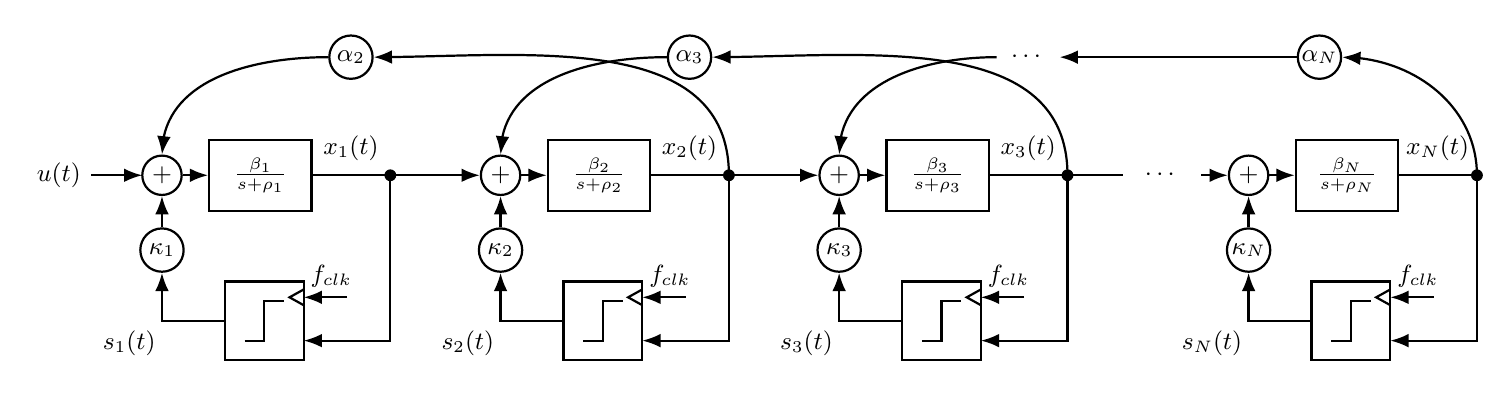
\begin{tikzpicture}[thick, font=\small]

  \tikzset{sum/.style={draw, circle, minimum size=0.5cm, inner sep=0pt},
           gain/.style={draw, circle, minimum size=0.55cm, inner sep=0pt},
           int/.style={draw, minimum width=1.3cm, minimum height=0.9cm}}

  \node[anchor=east] at (0.3,0) {$u(t)$};
  \draw[->] (0.3,0) -- (0.95,0);

  \foreach \x/\n in {1.2/1, 5.5/2, 9.8/3, 15.0/N} {
    \node[sum] (s\n) at (\x,0) {$+$};
    \node[int] (i\n) at (\x+1.25,0) {$\frac{\beta_{\n}}{s+\rho_{\n}}$};
    \draw[->] (s\n) -- (i\n);
    \coordinate (x\n) at (\x+2.9,0);
    \draw (i\n.east) -- (x\n);
    \fill (x\n) circle (0.075);
    \node[anchor=south] at (\x+2.4,0.05) {$x_{\n}(t)$};

    % local control: comparator, kappa, back into the summing node
    \node[gain] (k\n) at (\x,-0.95) {$\kappa_{\n}$};
    \draw[->] (k\n) -- (s\n);
    \draw (\x+0.8,-2.35) rectangle (\x+1.8,-1.35);
    \draw (\x+1.05,-2.1) -- (\x+1.3,-2.1) -- (\x+1.3,-1.6) -- (\x+1.55,-1.6);
    \draw (\x+1.8,-1.45) -- (\x+1.62,-1.55) -- (\x+1.8,-1.65);
    \draw[->] (\x+2.35,-1.55) -- (\x+1.8,-1.55);
    \node[anchor=south] at (\x+2.15,-1.55) {$f_{clk}$};
    \draw[->] (x\n) -- (\x+2.9,-2.1) -- (\x+1.8,-2.1);
    \draw[->] (\x+0.8,-1.85) -- (\x,-1.85) -- (k\n.south);
    \node[anchor=north east] at (\x+0.05,-1.85) {$s_{\n}(t)$};
  }

  % the chain
  \draw[->] (x1) -- (s2.west);
  \draw[->] (x2) -- (s3.west);
  \draw (x3) -- (13.4,0);
  \node at (13.9,0) {$\cdots$};
  \draw[->] (14.4,0) -- (sN.west);

  % leapfrog feedback, each state back over one stage
  \node[gain] (a2) at (3.6,1.5) {$\alpha_2$};
  \node[gain] (a3) at (7.9,1.5) {$\alpha_3$};
  \node at (12.2,1.5) {$\cdots$};
  \node[gain] (aN) at (15.9,1.5) {$\alpha_N$};
  \draw[->] (x2) to [out=90, in=0] (a2);
  \draw[->] (a2) to [out=180, in=90] (s1.north);
  \draw[->] (x3) to [out=90, in=0] (a3);
  \draw[->] (a3) to [out=180, in=90] (s2.north);
  \draw[->] (xN) to [out=90, in=0] (aN);
  \draw[->] (aN) -- (12.6,1.5);
  \draw[->] (11.8,1.5) to [out=180, in=90] (s3.north);

\end{tikzpicture}
\end{document}
